\newpage
\hypertarget{sec:Rules}{}
\section{Specifying TGG rules}
\genHeader

With our correspondence type defined in the TGG schema, we can now specify a set of \emph{TGG rules} to describe a language of graph
triples.

As discussed in \Cref{sec:nutshell}, a TGG rule is quite similar to a story pattern, following a \emph{precondition-postcondition} format.
This means we'll need to state:

\begin{itemize}

\item \textbf{Context:} What must be matched (\idest, under which conditions can a rule be applied; shown as \emph{black} elements)

\item \textbf{Modifications:} What is to be created when the rule is applied (\idest, which objects and links must exist upon exit; shown as \emph{green} elements)

\end{itemize}

\vspace{0.5cm}

Note that the rules of a TGG only describe the simultaneous \emph{build-up} of source, correspondence, and target models.
Unlike story diagrams, they do not delete or modify existing elements---you will never find a red element in an eMoflon TGG.
In other words, TGG rules are \emph{monotonic}.\define{Monotonicity}
This might seem surprising at first, and you might even think this is a terrible restriction. 
The intention is that a TGG should only specify a consistency relation, and \emph{not} the forward and backward transformations
directly, which are derived automatically. 
In the end, modifications are not necessary on this level but can, of course, be induced in certain operationalizations of the TGG.

Let's quickly think about what rules we need in order to successfully transform a learning box into a dictionary. 
We need to first take care of the \texttt{Box}
and \texttt{Dictionary} structures, where \texttt{Box} will need at least one \texttt{Partition} to manipulate its \texttt{Card}s.
If more than one is created, those partitions will need to have appropriate \texttt{next} and \texttt{previous} links. 
Conversely, given that a \texttt{dictionary} is unsorted, there are no
counterparts for partitions. 
A second rule will be needed to transform \texttt{Card}s into \texttt{Entries}.
More precisely, a one-to-one correspondence must be
established (\idest, one \texttt{Card} implies one \texttt{Entry}), with suitable concatenation or splitting of the contents (based on the transformation direction), and some mechanism to assign difficulty levels to each \texttt{Entry} or initial position of each \texttt{Card}.

\newpage
\hypertarget{rules vis}{}
\subsection{BoxToDictionaryRule}
\genHeader

\begin{stepbystep}

\item Select the created subpackage \texttt{src/org.moflon.tgg.mosl.rules} (Step 1 in \Cref{ea:create_tgg_rule}) and click on the wizard \menuPath{Create new TGG rule} (\eMoflonCreateTGGRuleIcon, Step~2).
In the dialogue that pops up, enter \texttt{BoxToDictionaryRule} as the name of the TGG rule to be created.
Open the newly created file.

\begin{figure}[htbp]
\begin{center}
  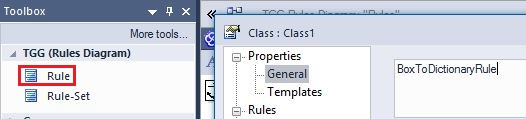
\includegraphics[width=0.8\textwidth]{../../org.moflon.doc.handbook.04_tripleGraphTransformations/4_rules/visRImages/ea_TGGNewRule.jpg}
  \caption{Creating a TGG rule}
  \label{ea:create_tgg_rule}
\end{center}
\end{figure}

\begin{figure}[htbp]
\begin{center}
  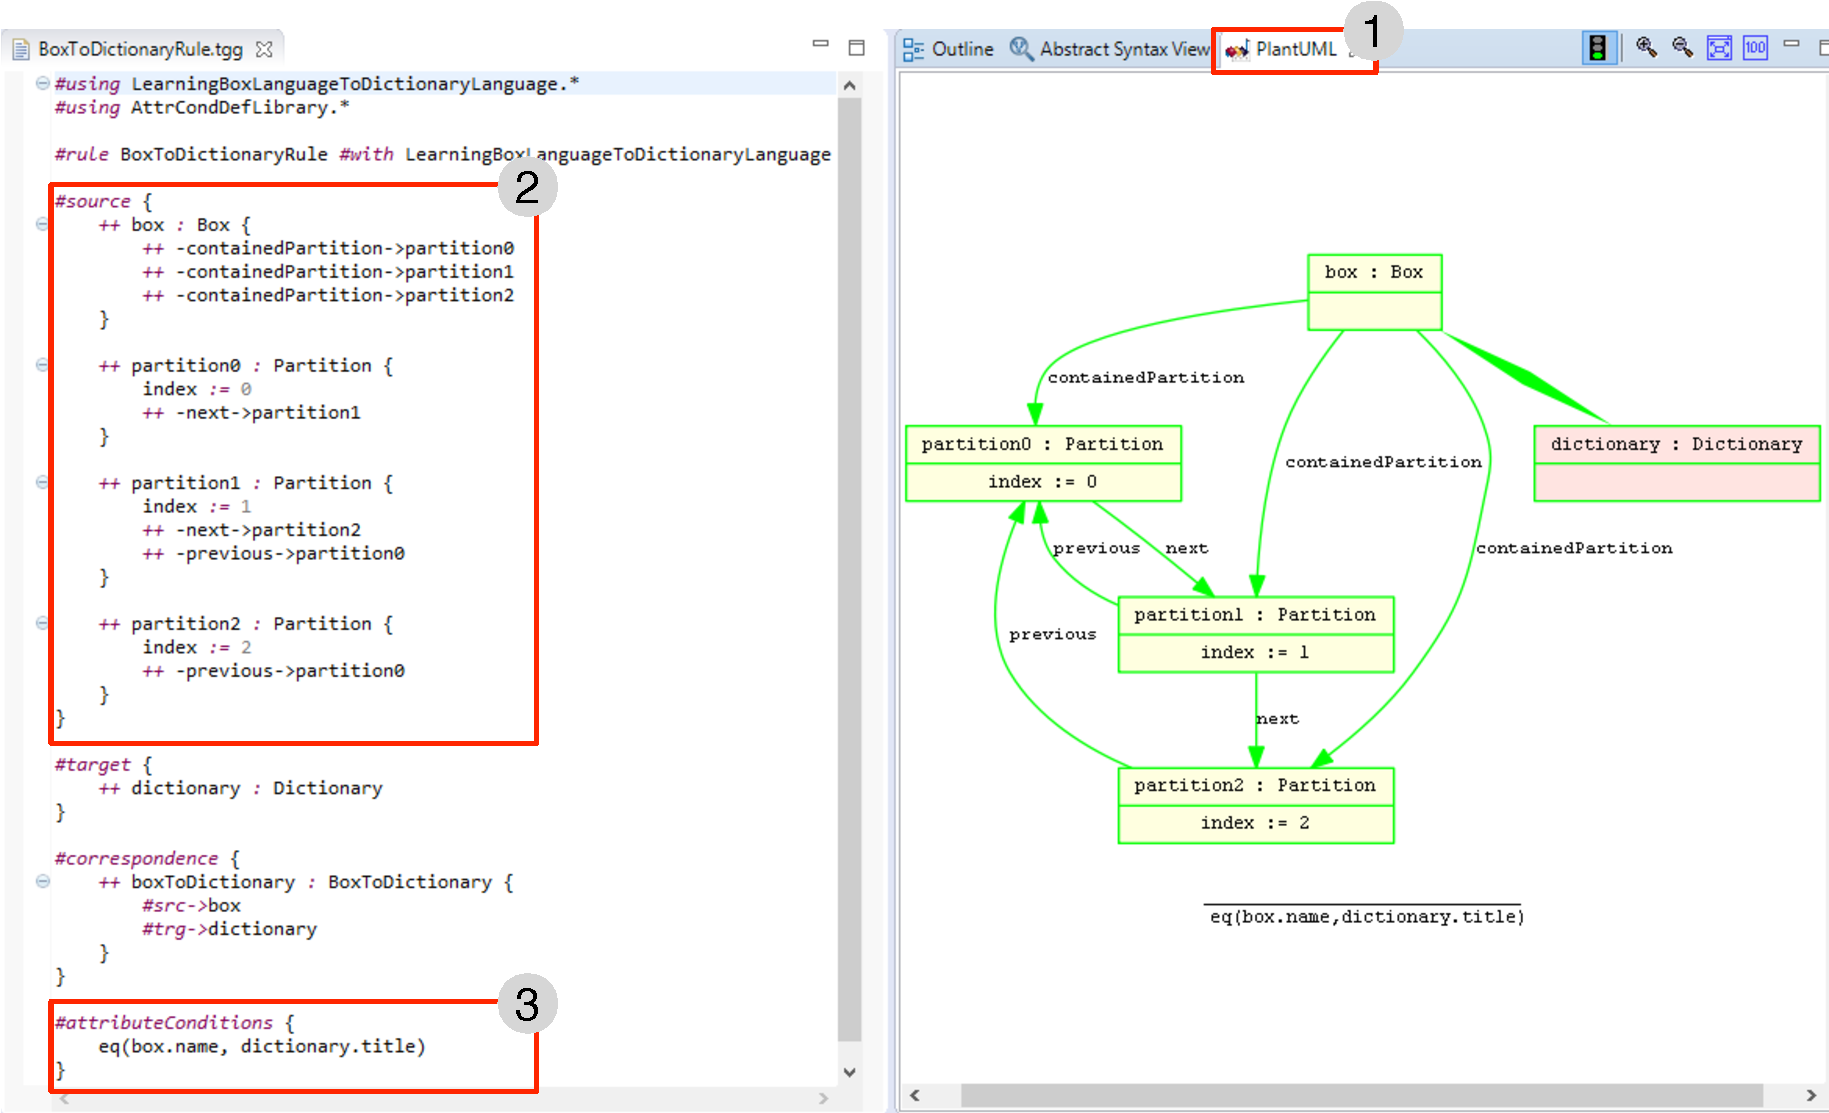
\includegraphics[angle=90,width=\textwidth]{../../org.moflon.doc.handbook.04_tripleGraphTransformations/4_rules/visRImages/ea_BoxToDictionaryRuleComplete.pdf}
  \caption{Complete TGG rule diagram for \texttt{BoxToDictionaryRule}}
  \label{ea:boxtodictionaryrule_complete}
  \end{center}
\end{figure}

\item  Ensure that you open the \texttt{PlantUML} view (Step 1 in \Cref{ea:boxtodictionaryrule_complete}) as it provides a helpful visualisation of the current TGG rule opened in the editor.
To prevent slowing you down, the view is only updated when you save \emph{and} change your cursor position.

Elements in the source domain have a yellow background, while target elements have a peach background.
Basic UML object diagram syntax is used, extended with colours to represent created elements (green outline) and context elements (black outline).

\texttt{BoxToDictionaryRule} is a so-called \emph{island rule} and only has created elements.
For presentation purposes, correspondence links are abstracted from in the visualisation and are depicted as bands (\eg, between \texttt{box} and \texttt{dictionary}).
The rule we want to specify creates a minimal dictionary (just a \texttt{Dictionary} node), and a minimal box, which is a bit more interesting as it consists already of three correctly connected partitions.
Any structure less than this is not a valid learning box.

\item The textual syntax we use is pretty straightforward:  every domain has a scope (\moslTggCode{\#source}, \moslTggCode{\#target}, and \moslTggCode{\#correspondence}), and there is a final scope for so called attribute conditions, which express how attribute values relate to each other.
The domain scopes contain again scopes for each \emph{object variable} in the rule (e.g., \texttt{box}) and these scopes then contain outgoing \emph{link variables} (\eg, \moslTggCode{-contained\-Partition->}), as well as inline attribute conditions (\eg, \moslTggCode{index := 0}).
Go ahead and specify the source scope as depicted in Step 2 of \Cref{ea:boxtodictionaryrule_complete}.
Notice how the \moslTggCode{++} operator is used to mark object and link variables as created or context variables.
Try removing and adding it and see how the visualisation changes.  
As always, let the editor help you by pressing \shortcut{Ctrl+Space} as often as possible.

\item Specify the \moslTggCode{#correspondence} and \moslTggCode{#target} scopes accordingly and make sure your rule (and its visualisation) closely resembles \Cref{ea:boxtodictionaryrule_complete}.

\item To complete our first rule, specify an attribute condition (inside the \moslTggCode{#attributeConditions} scope) to declare that the name of the box and the title of the dictionary are always to be equal.
As depicted in Step 3 \Cref{ea:boxtodictionaryrule_complete}, this can be accomplished using an \texttt{eq} condition.
We provide a standard library of such attribute conditions (press \shortcut{F3} on the constraint to jump to the library file), but it is also possible to extend this library with your own attribute conditions.
We'll see how to do this in a moment.
\end{stepbystep}

Fantastic work! The first rule of our transformation is complete! 
If you are in hurry, you could jump ahead and proceed directly to \Cref{sect:TGGs_in_Action}: TGGs in Action. 
There you can transform a box to a dictionary and vice-versa, but please be aware that your specified TGG (with just one rule) will only be able to cope with completely empty boxes and dictionaries. 
Handling additional elements (i.e., cards in the learning box and entries in the dictionary) requires a second rule.
We intend to specify this next.

\subsection{CardToEntryRule}

Our next goal is to be able to handle \texttt{Card} and \texttt{Entry} elements. 
The new thing here is that it will require a pre-condition -- you should not be able to transform these child elements (cards and entries) unless certain structural conditions (their parents exist and are related) are met. 
In other words, we need a rule that demands an already existing \texttt{box} and \texttt{dictionary}. 
It will need to combine `black' and `green' variables! 

\begin{stepbystep}

\item As we'll be connecting cards and entries, we need a new correspondence type.
Open the TGG schema (\filename{Schema.tgg}) and add a new correspondence type \moslTggCode{CardToEntry} connecting a \texttt{Card} (\moslTggCode{#src}) and an \texttt{Entry} (\moslTggCode{#trg}).

\item Create a new TGG rule with \texttt{CardToEntryRule} its name, and specify the rule as depicted in \Cref{ea:cardtoentry_1}.
\end{stepbystep}

Your diagram should now resemble \Cref{ea:cardtoentry_1}. 
We're not done yet though, we still need to handle attributes!
To understand why, consider the current rule and ask yourself  \emph{which} partition is meant.
Exactly!  This is currently not specified, so \emph{any} partition can be taken when applying the rule.
eMoflon would actually collect all applicable rules (one for every partition) and consult a configuration component to decide which rules should be taken.
The default component just chooses randomly, but you could override this and, \eg, pop up a dialogue asking the user which partition to use.
Although this could be an interesting solution, we'll see how to fully specify things using extra attribute conditions.

\begin{figure}[htbp]
  \begin{center}
    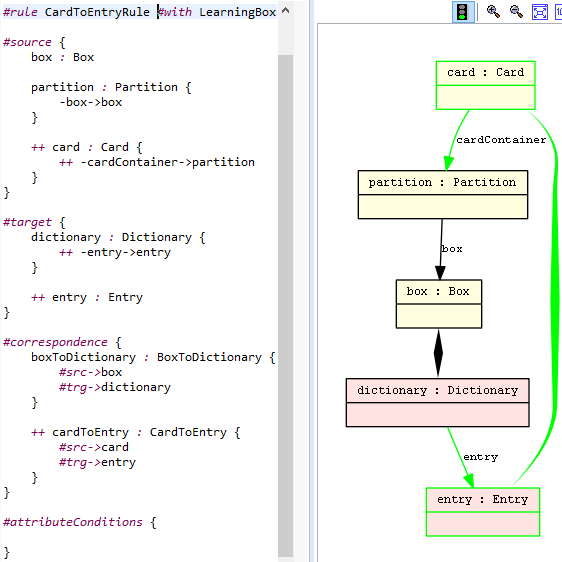
\includegraphics[width=\textwidth]{../../org.moflon.doc.handbook.04_tripleGraphTransformations/4_rules/visRImages/ea_cardToEntryRule.PNG}
    \caption{\texttt{CardToEntryRule} without attribute manipulation}
    \label{ea:cardtoentry_1}
  \end{center}
\end{figure}

On the way to handling all attributes, let's first start with the relatively easy case of specifying how every \moslTggCode{entry.content}, \moslTggCode{card.back}, and \moslTggCode{card.face} relate to each other.
We should probably combine the front and back of each card as a single content attribute of an entry and, in the opposite direction, split the content into \texttt{card.back} and \texttt{card.face}.

So let's define \moslTggCode{entry.content} as: \moslTggCode{<word>:<meaning>}. 
Therefore, \moslTggCode{card.back} should be \moslTggCode{Question:<word>} and similarly, \moslTggCode{card.face} should be \moslTggCode{Answer:<meaning>}. 

\begin{stepbystep}
\item Luckily, we have two library attribute conditions, \texttt{addPrefix} and \texttt{concat} to help us with this.
Add the following to the \moslTggCode{#attributeConditions} scope of your rule:

\moslTggCode{addPrefix("Question ", word, card.back)}\\  
\moslTggCode{addPrefix("Answer ", meaning, card.face)}\\
\moslTggCode{concat(":", word, meaning, entry.content)}

\moslTggCode{Question} and \moslTggCode{Answer} are EString literals, \moslTggCode{word} and
\moslTggCode{meaning} are local variables, and \moslTggCode{card.face}, \moslTggCode{card.back}, and \moslTggCode{entry.content} are attribute expressions.

\item Our final task is now to specify where a new \moslTggCode{card} (when transformed from an \moslTggCode{entry}) should be placed.  
We purposefully created three partitions to match the three difficulty levels, but if you check the available library constraints, there is nothing that can directly implement this specific kind of mapping. 
We will therefore need to create our own attribute condition to handle this.

\item Open the TGG schema (\filename{Schema.tgg}), and define a new attribute condition in the \moslTggCode{#attributeConditions} scope. 
Name it \moslTggCode{indexToLevel}, and enter the values given in \Cref{ea:create_new_constraint}.

\begin{figure}[htbp]
\begin{center}
  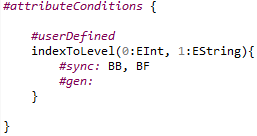
\includegraphics[width=0.45\textwidth]{../../org.moflon.doc.handbook.04_tripleGraphTransformations/4_rules/visRImages/ea_uniqueConstraint.PNG}
  \caption{Specifying the new attribute condition \moslTggCode{indexToLevel}}
  \label{ea:create_new_constraint}
\end{center}
\end{figure}
\FloatBarrier

\item Please note that this is just a \emph{specification} of a custom attribute condition -- we still need to actually implement it in Java! 
As we're so close to finishing this TGG rule, however, let's complete it first before we work out the exact meaning of the mysterious adornments (those funny \texttt{BB}, \texttt{BF}, \dots) and parameters (\texttt{0:EInt} and \texttt{1:EString}) of the attribute condition. 
For now, just make sure you enter the exact values in \Cref{ea:create_new_constraint}. 

\item We can now use this new attribute condition \moslTggCode{indexToLevel} just like any of the library attribute conditions.
Add the following code to the \moslTggCode{#attributeConditions} scope of the \texttt{CardToEntryRule} to express that the relationship between the index of the partition containing the new card, and the level of the new entry, is defined by our new attribute condition:

\moslTggCode{indexToLevel(partition.index, entry.level)}
\end{stepbystep}

If everything has been done correctly up to this point, your project should save and build.
The generated code will have some compilation errors (Step 1 in Fig.~\ref{eclipse:tggGenerated}) as Eclipse does not know where to access the generated code for the imported source and target ecore files (these could also be supplied from jars or installed plugins).
In our case the generated code is in the respective source and target projects so let's communicate this to Eclipse.

\begin{stepbystep}

\item Open the \texttt{MANIFEST.MF} file (Step 2 in Fig.~\ref{eclipse:tggGenerated}) and choose the \texttt{De\-pen\-den\-cies} tab (Step 3).

\item Choose both source and target projects (\texttt{DictionaryLanguage}, \texttt{Learning\-Box\-Language}, Step 4) as dependencies and click \texttt{OK}.
All compilations errors should now be resolved.
\end{stepbystep}

\begin{figure}[htb]
\begin{center}
  \includegraphics[width=0.8\textwidth]{../../org.moflon.doc.handbook.04_tripleGraphTransformations/4_rules/eclipse_generatedTGG.pdf}
  \caption{Add source and target projects as dependencies}
  \label{eclipse:tggGenerated}
\end{center}
\end{figure}

Great work! All that's left to do is implement the \texttt{indexToLevel} constraint, and give your transformation a test run.


\hypertarget{subsec:IndexToLevel}{}
\subsection{Implementing IndexToLevel}
\genHeader

If everything has been done correctly up to this point, your project should save and build (hit the hammer symbol in the eMolfon task bar).
The generated code will have some compilation errors (Step 1 in \Cref{eclipse:tggGenerated}) as Eclipse does not know where to access the generated code for the imported source and target ecore files (these could also be supplied from jars or installed plugins).
In our case the generated code is in the respective source and target projects so let's communicate this to Eclipse.

\begin{enumerate}

\item[$\blacktriangleright$] Open the \texttt{MANIFEST.MF} file (Step 2 in \Cref{eclipse:tggGenerated}) and choose the \texttt{De\-pen\-den\-cies} tab (Step 3).

\item[$\blacktriangleright$] Choose both source and target projects (Step 4) as dependencies and click \texttt{OK}.
All compilations errors should now be resolved.
\end{enumerate}

\begin{figure}[htb]
\begin{center}
  \includegraphics[width=0.8\textwidth]{eclipse_generatedTGG}
  \caption{Add source and target projects as dependencies}
  \label{eclipse:tggGenerated}
\end{center}
\end{figure}

Our TGG still isn't yet complete. 
While we've declared and actually used our custom \texttt{indexTolevel} attribute condition, we haven't actually implemented it yet. 
Let's quickly review the purpose of attribute conditions.

Just like patterns describing \emph{structural} correspondence, \emph{attribute conditions} can be automatically \emph{operationalized} as required, e.g., for a forward transformations. 
Even more interesting, a set of attribute conditions might have to be ordered in a specific way depending on the direction of the transformation.
Enforcing the conditions might involve checking existing attribute values, or setting these values appropriately.

For built-in \emph{library} attribute conditions such as \emph{eq}, \emph{addPrefix} and \emph{concat}, you do not need to worry about these details and can just focus
on expressing what should hold. 
Everything else is handled automatically.

In some cases however, a required attribute condition might be problem-specific, such as our \emph{indexToLevel}. 
There might not be any fitting combination of library attribute conditions to express the consistency condition, so a new attribute condition type must be declared and implemented.

There is a list of \emph{adornments} in the declaration which specify the cases for which the attribute condition can be operationalized. 
Each adornment consists of a \texttt{B} (bound) or \texttt{F} (free) variable setting for each argument of the attribute condition. 
This might sound a bit complex, but it's really quite simple, especially in the context of our example:

\begin{description}

\item[BB] indicates that the \texttt{partition.index} and \texttt{entry.level} are both \emph{bound}, i.e., they already have assigned values.
In this case, the \emph{operation} must check if the assigned values are valid and correct.

\item[BF] indicates that \texttt{partition.index} is \emph{bound} and \texttt{entry.level} is \emph{free}, i.e., the operation must determine and assign the correct value to \texttt{entry.level} using \texttt{partition.index}.

\item[FB] would indicate that \texttt{partition.index} is \emph{free} and \texttt{entry.level} is \emph{bound}, i.e., the operation must determine and assign the correct value to \texttt{parti\-tion.in\-dex} using \texttt{entry.level}.

\item[FF] would indicate that both \texttt{partition.index} and \texttt{entry.level} are \emph{free} and we have to somehow generate consistent values out of thin air.

\end{description}

As \texttt{partition} is a context element in the rule (the partition is always bound in whatever direction), \textbf{FF} and \textbf{FB} are irrelevant cases and we do not need to declare or implement what they mean.
For the record, note that adornments can be declared as either \texttt{\#gen} or \texttt{\#sync}.
The reason is that it might make sense to restrict some adornments (typically \textbf{FF} cases) to only when generating models.
Using \textbf{FF} cases for synchronisation might possibly makes sense, but most of the time it would be weird to generate random values during a forward or backward synchronisation.  

At compile time, the set of attribute conditions for every TGG rule is ``solved'' for each case by
operationalizing all constraints and determining a feasible sequence in which the operations can be executed, compatible to the declared adornments of each attribute condition. 
If the set of attribute conditions cannot be solved, an exception is thrown at compile time.

Now that we have a better understanding behind the construction of attribute conditions, let's implement \texttt{indexToLevel}.

\begin{itemize}
\item[$\blacktriangleright$] Locate and open \texttt{IndexToLevel.java} under ``src/csp.constraints'' in \texttt{LearningBoxToDictionaryIntegration}.

\item[$\blacktriangleright$] As you can see, some code has been generated in order to handle the current unimplemented state of \texttt{IndexToLevel}. 
Use the code depicted in \Cref{code:indexToLevel} to replace this default implementation.\footnote{Depending of course on your pdf viewer, copy and pasting this code should work.}

\begin{figure}[htb]
\begin{verbatim}
package csp.constraints;

import java.util.Arrays;
import java.util.List;
import org.moflon.tgg.language.csp.Variable;
import org.moflon.tgg.language.csp.impl.TGGConstraintImpl;

public class IndexToLevel extends TGGConstraintImpl {

    private static List<String> levels = 
      Arrays.asList(new String[] {"master","advanced","beginner"});

    public void solve(Variable var_0, Variable var_1) {
        int index = ((Integer) var_0.getValue()).intValue();
        int normalisedIndex = Math.min(Math.max(0, index), 2);
        String bindingStates = getBindingStates(var_0, var_1);
        
        switch (bindingStates) {
        case "BB":
            String level = (String) var_1.getValue();
            setSatisfied(levels.get(normalisedIndex).equals(level));
            break;
        case "BF":
            var_1.bindToValue(levels.get(normalisedIndex));
            setSatisfied(true);
            break;
        }}}
\end{verbatim}
  \caption{Implementation of our custom \texttt{IndexToLevel} constraint}
  \label{code:indexToLevel}
\end{figure}

\end{itemize}

To briefly explain, the \texttt{levels} list contains difficulty level at positions 0, 1, or 2 in the list, which correspond to our three partitions in the learning box. 
You'll notice that instead of setting ``master'' to 2, it has rather been set to match the first 0th partition. 
Unlike an \texttt{entry} in \texttt{dictionary}, the position of each \texttt{card} in \texttt{box} is \emph{not} based on difficulty, but simply how it has been moved as a result of the user's correct and incorrect guesses. 
Easy cards are more likely to be in the final partition (due to moving through the box quickly) while challenging cards are most likely to have been returned to (and currently to be at) the starting position, i.e., the 0th partition.

In the \texttt{solve} method, the index of the matched partition in the rule is first of all normalised (negative values do not make sense, and we handle all partitions  after partition 2 in the same way).
A switch statement is then used, based on whichever adornment is currently the case, to enforce or check the condition. 

For \texttt{BB} we check if the normalised index of the partition corresponds to the difficulty level of the card.
For \texttt{BF}, the normalised index is used to set the appropriate difficulty level of the card.

%%% Local Variables: 
%%% mode: latex
%%% TeX-master: "../src/TGG_mainFile"
%%% End: 



%%% Local Variables: 
%%% mode: latex
%%% TeX-master: "../src/TGG_mainFile"
%%% End: 
